\documentclass[border=10pt]{standalone}

\usepackage{tikz}
\usepackage{tikzsymbols}
\usetikzlibrary{calc,patterns,shapes.geometric}

\def\centerarc[#1](#2)(#3:#4:#5){\draw[#1] ($(#2)+({#5*cos(#3)},{#5*sin(#3)})$) arc (#3:#4:#5);}

\begin{document}
	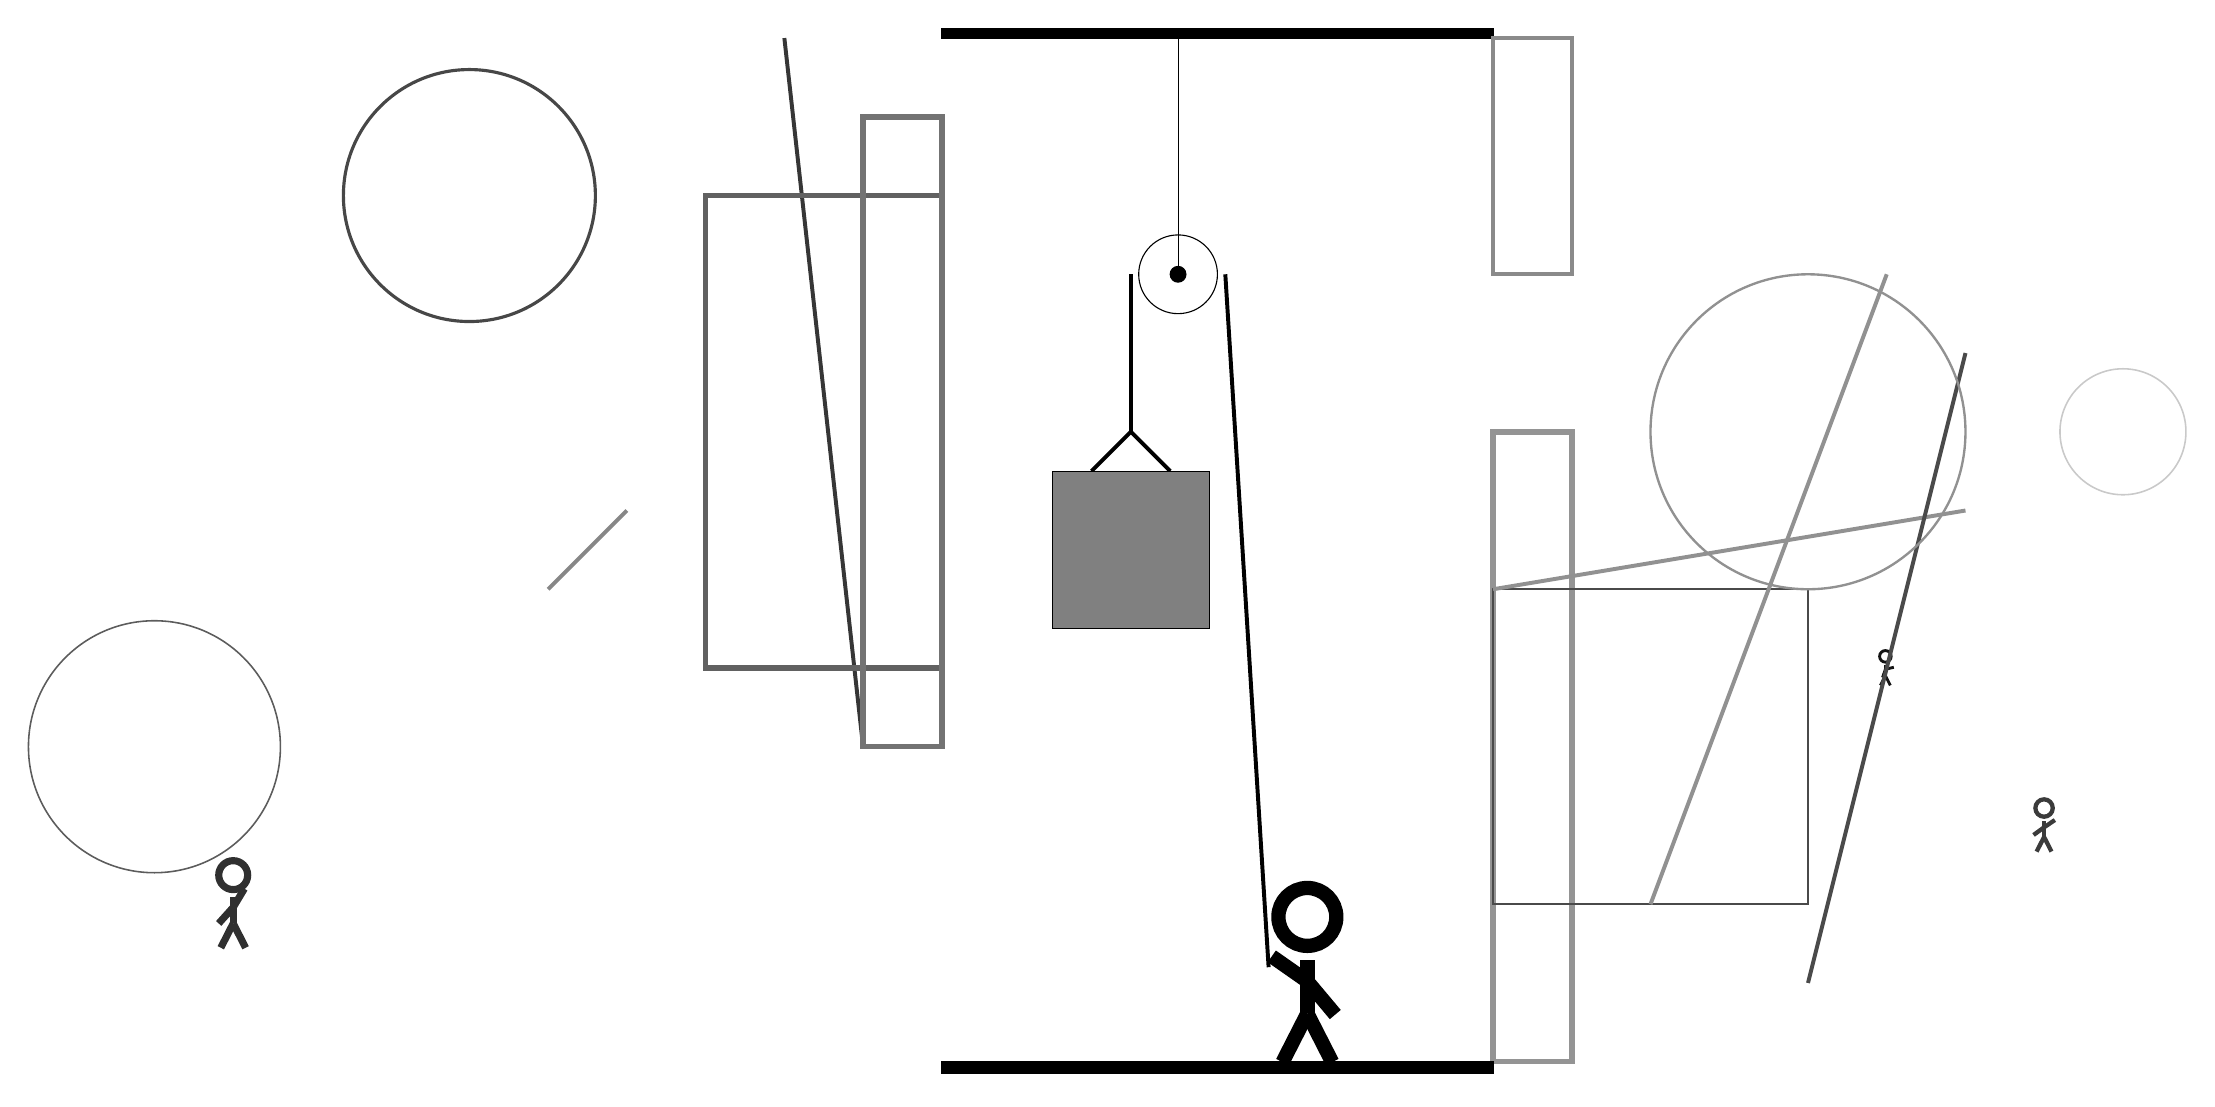
\begin{tikzpicture}
		%%%%% START %%%%%
		
		\draw[fill=black] (-2, 10) rectangle (5, 10.125);
		
		\draw (1, 7) circle (0.5);
		\draw[fill=black] (1, 7) circle (0.1);
		\draw (1, 10) -- (1, 7);
		
		\draw[line width=0.5mm] (-0.1, 4.5) -- (0.4, 5.0) -- (0.9, 4.5);
		\draw[fill=black!50] (-0.6, 4.5) rectangle (1.4, 2.5);
		
		\draw [line width=0.4mm, color=black!72](-8, 8) circle (1.6);
		
		\draw[line width=0.5mm, color=black!79](-3, 1) -- (-4, 10);
		\node[line width=0.4mm, color=black!92] at (10, 2) {\Strichmaxerl[2][71][13]};
		\draw[line width=0.7mm, color=black!62] (-2, 2) rectangle (-5, 8);
		\draw[line width=0.7mm, color=black!42] (6, -3) rectangle (5, 5);
		\node[line width=0.5mm, color=black!77] at (12, 0) {\Strichmaxerl[3][36][34]};
		\draw [line width=0.2mm, color=black!21](13, 5) circle (0.8);
		\draw [line width=0.2mm, color=black!64](-12, 1) circle (1.6);
		\node[line width=0.7mm, color=black!81] at (-11, -1) {\Strichmaxerl[5][48][59]};
		
		\draw[line width=0.5mm, color=black!46] (5, 7) rectangle (6, 10);
		\draw[line width=0.3mm, color=black!71] (5, -1) rectangle (9, 3);
		\draw[line width=0.5mm, color=black!43](5, 3) -- (11, 4);
		\draw[line width=0.5mm, color=black!71](9, -2) -- (11, 6);
		
		\draw[line width=0.7mm, color=black!55] (-3, 1) rectangle (-2, 9);
		\draw [line width=0.3mm, color=black!43](9, 5) circle (2.0);
		\draw[line width=0.5mm, color=black!47](-7, 3) -- (-6, 4);
		
		\draw[line width=0.5mm, color=black!43](7, -1) -- (10, 7);
		
		\draw[line width=0.5mm] (0.4, 7) -- (0.4, 5.0);
		\centerarc[line width=0.5mm](1, 7)(0:180:0.6);
		\draw[line width=0.5mm](1.6, 7) -- (2.15, -1.8);
		
		\node at (2.6, -1.9) {\Strichmaxerl[10][-35][-50]};
		
		\draw[fill=black] (-2, -3) rectangle (5, -3.15);
		
		%%%%% END %%%%%
	\end{tikzpicture}
\end{document}